\section{Theory}
\label{sec:theory}

The following is a short summary of the used equations, which were adopted
from chapter 3 of the course book~\cite{Bonet2008}.
Unless stated otherwise, the uppercase letters refer to the initial (reference)
configuration of the problem, while the lowercase ones refer to the current
configuration. The boldface letters denote vectors, matrices and tensors.

For a given load, solving the problem implies finding a configuration that
simultaneously satisfies both the global (system) equilibrium equations and
the constitutive equations.
The equilibrium equations are expressed in terms of the residual (out-of-balance)
vector \(\bm{R} (\bm{x})\) as the balance between internal and external forces:
\begin{equation}
  \bm{R} (\bm{x}) = \bm{T} (\bm{x}) - \bm{F} = \bm{0},
\end{equation}
where \(\bm{x} =\left[ \bm{x}_{1}, \bm{x}_{2}, \cdots, \bm{x}_{N} \right]^{\text{T}}\)
is the vector of current nodal positions;
\(\bm{T} =\left[ \bm{T}_{1}, \bm{T}_{2}, \cdots, \bm{T}_{N} \right]^{\text{T}}\) is
the vector of internal nodal forces;
\(\bm{F} =\left[ \bm{F}_{1}, \bm{F}_{2}, \cdots, \bm{F}_{N} \right]^{\text{T}}\) is
the vector of external nodal forces, where it is assumed to be independent
of the current nodal positions \(x\) (generally this is not true);
and \(N\) is the number of nodes.

\subsection{Hyperelasticity}
\label{sec:hyperelasticity}

In the case of hyperelastic material behaviour of a rod, i.e.\ material whose
strain energy per unit volume \(V\) does not depend on the path taken by the rod as
it moved from initial length \(L\) to the current length \(l\), the internal
truss forces \(\bm{T}_{a}\) and \(\bm{T}_{b}\) can be computed as
\begin{equation}
  \bm{T}_{b} = \frac{V E}{l} \ln \left( \frac{l}{L} \right) \bm{n}
             = \tau \frac{V}{l} \bm{n}, \quad
  \bm{T}_{a} = - \bm{T}_{b}.
\end{equation}
Here, a Young's modulus like constant \(E\) has been used to relate Kirchhoff
stress \(\tau = E \varepsilon = \sigma v / V\) to logarithmic strain
\(\varepsilon = \ln(l/L)\).

Finding equilibrium position is carried out using Newton-Raphson method, which
involves linearisation of the equilibrium equations. The linearisation yields
the directional derivative \(D \bm{T}^{(e)} (\bm{x}^{(e)}) [\bm{u}^{(e)}]\),
which gives the
expression for the tangent stiffness matrix:
\begin{equation}
  D \bm{T}^{(e)} (\bm{x}^{(e)}) [\bm{u}^{(e)}] = \bm{K}^{(e)} \bm{u}^{(e)} =
  \begin{bmatrix}
    \bm{K}_{aa}^{(e)} & \bm{K}_{ab}^{(e)} \\
    \bm{K}_{ba}^{(e)} & \bm{K}_{bb}^{(e)}
  \end{bmatrix}
  \begin{bmatrix}
    \bm{u}_{a} \\
    \bm{u}_{b}
  \end{bmatrix}
\end{equation}
with
\begin{align}
  \bm{K}_{aa}^{(e)} &= \bm{K}_{bb}^{(e)} =\left( \frac{V}{v}
                      \frac{d \tau}{d \varepsilon} \frac{a}{l} -
                      \frac{2 \sigma a}{l} \right)
                      \bm{n} \otimes \bm{n} + \frac{\sigma a}{l} \bm{I} \\
  \bm{K}_{ab}^{(e)} &= \bm{K}_{ba}^{(e)} = - \bm{K}_{aa}^{(e)},
\end{align}
where \(d \tau / d \varepsilon = E\) is the elastic material tangent modulus.

\subsection{Rate-independent plasticity}
\label{sec:plasticity}

In the case of rate-independent finite strain plasticity with isotropic hardening,
the stress is defined via elastic strain \(\varepsilon_{e}\):
\begin{align}
  \tau &= E \varepsilon_{e} = E \left( \varepsilon - \varepsilon_{p} \right) \\
  \varepsilon_{p} &= \int_{0}^{t} \dot{\varepsilon}_{p} dt \label{eq:plastic-strain}
\end{align}

The onset of plastic deformation is governed by the yield condition, which for the
problem at issue is
\begin{equation}
  f (\tau, \bar{\varepsilon}_{p}) = \left| \tau \right| - \left(
    \tau_{y}^{0} + H \bar{\varepsilon}_{p} \right) \leq 0, \quad 
  \bar{\varepsilon}_{p} \geq 0, 
\end{equation}
where \(\tau_{y}^{0}\) is the initial yield stress,
\(\bar{\varepsilon}_{p}\) is the hardening parameter and \(H\) is a material
property called plastic modulus.
At its simplest, the hardening parameter is defined as the accumulated absolute
plastic strain occurring over time:
\begin{equation}
  \bar{\varepsilon}_{p} = \int_{0}^{t} \dot{\bar{\varepsilon}}_{p} dt,
  \quad \dot{\bar{\varepsilon}}_{p} = \left| \dot{\varepsilon}_{p} \right|,
  \quad \dot{\varepsilon}_{p} = \dot{\gamma} \frac{\partial f}{\partial \tau},
\end{equation}
where \(\dot{\gamma}\) is plastic multiplier.

In a computational setting the time integration of \eqref{eq:plastic-strain} can
only be performed approximately from a finite sequence of values determined at
different time steps.
In order to satisfy the yield condition exactly at each incremental time step,
a return-mapping algorithm described in figure~\ref{fig:return-mapping} is used,
which employs incremental kinematics (see figure~\ref{fig:incr-kinematics}).
\begin{figure}[th]
  \begin{subfigure}[t]{0.38\textwidth}
    \centering
    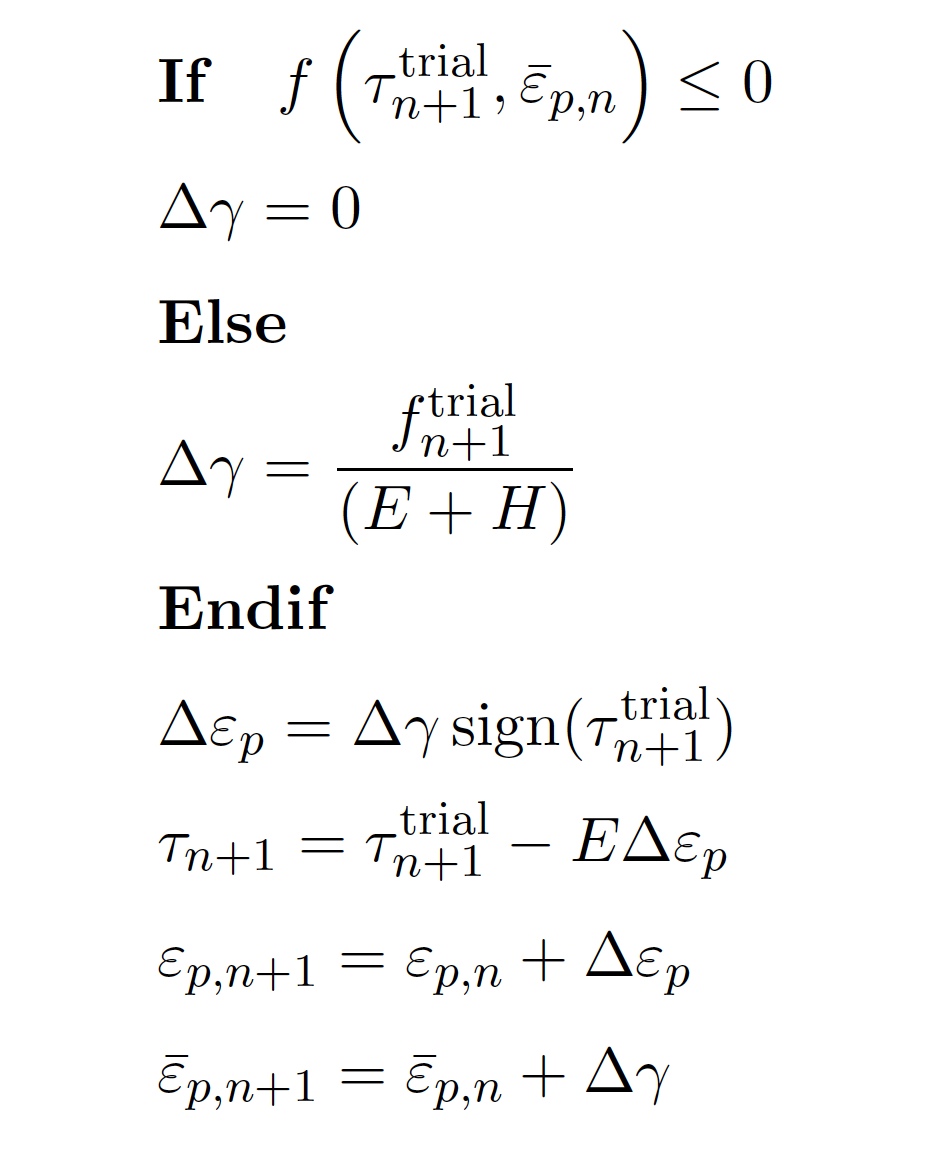
\includegraphics[width=\textwidth]{return_mapping.png}
    \caption{Return-mapping algorithm.}
    \label{fig:return-mapping}
  \end{subfigure}
  ~
  \begin{subfigure}[t]{0.56\textwidth}
    \centering
    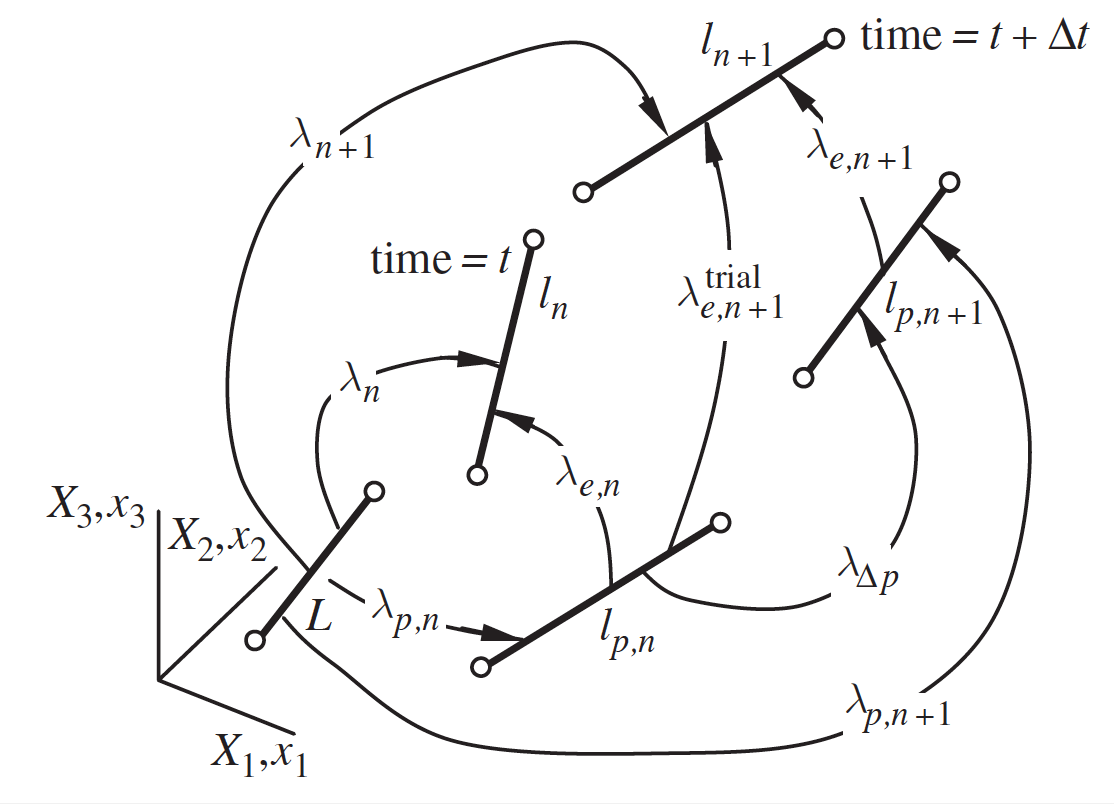
\includegraphics[width=\textwidth]{incremental_kinematics.png}
    \caption{Incremental kinematics. \(\lambda = l / L\).}
    \label{fig:incr-kinematics}
  \end{subfigure}
  \caption{Two figures from \cite{Bonet2008}.}
\end{figure}

The last matter to be addressed in the presence of plasticity is the material
tangent modulus \(d \tau / d \varepsilon\).
The tangent modulus derived from incremental considerations is generally not
the same as the one obtained from the rate equations.
The reason is that the incremental change in stress imposed by the chosen
return-mapping algorithm is different from the continuous change in stress
stemming from the rate equations.
That is why the algorithmic tangent modulus is used:
\begin{equation}
  \frac{d \tau_{n+1}}{d \varepsilon_{n+1}} = \frac{E H}{E + H}
\end{equation}
When plasticity occurs, this replaces the elastic tangent stiffness
\(d \tau / d \varepsilon = E \).

%%% Local Variables:
%%% mode: latex
%%% TeX-master: "../main"
%%% End:
